The XY model has been studied with various approaches, the one taken in this
dissertation is a Monte Carlo simulation that will be implemented to compute
physical observables from which it will be attempted to estimate some critical
exponents. A brief introduction on theory of Monte Carlo simulations will be
followed by a description of this particular implementation and finally the 
results obtained will be illustrated.

\section{Theory}

The main idea of Monte Carlo simulations is to sample a quantity of interest,
treating it as a random variable even if in principal this quantity could be
obtained deterministically. This kind of probabilistic approach, instead of the
deterministic one, becomes useful when the deterministic evaluation via numerical
means results impossible. In physics this usually happens when numerical 
calculations in high dimensions are required, as in evaluation of integrals in 
multiple dimensions, and the computational cost in time scale as $N^2$ or in 
gerenal as a higher power of $N$, with $N$ being the number of dimensions.

Monte Carlo methods are based on the law of large numbers and on the central limit
theorem which states that the expected value of some random variable can be obtained
by the sample mean of indipendent samples of the variable. Then the central problem
of a Monte Carlo algorithm becomes sampling the variables of interest in a
indipendent and representative way.

In phisics and mathematics the algorithm mostly used to accomplish the requirements
needed is the so called Markov chain Monte Carlo sampler. The Markov chain 
\footnote{see \url{https://en.wikipedia.org/wiki/Markov_chain_Monte_Carlo}} is 
constructed based on the target sample distribution and the sampling of the states,
composing the chain, will approach the desired distribution in the limit of an 
infinite chain.

Finally the algorithm that puts all of these concepts togheter is the
Metropolis-Hastings algorithm. \footnote{Check the original work of Metropolis
and Rosenbluth spouses (\cite{Metropolis1953}) that inspired the invention of the
Metropolis-Hastings algorithm} This algorithm samples any random variable
provided that the probability density function $P(x)$, or a function proportional
to it, is known. Being  based on a Markov chain implicates that every sample is generated
based on the sample generated before, then the sample is accepted or not on 
probabilistic considerations built on $P(x)$. In case the new sample proposal
is rejected, the old sample value is retained and counted as a new sample on which
the values of observables will be computed again.

In the case of a lattice, as in the XY model, starting from a random spins' configuration,
the canonical distribution, coming from canonical ensemble theory, is used to determine which
configuration utilize to compute observables' values. The canonical
distribution is defined as
\begin{equation}
P(\{\sigma_i\}) = \frac{\exp(-\beta H(\{\sigma_i\}))}{Z}
\end{equation}
where $\{\sigma_i\}$ is the spins' configuration and $Z$ is the partition function.

Then in every Metropolis step a new candidate sample is created and the 
probabilities of the configuration are compared using the ratio between them
\begin{equation}
A = \frac{P(\{\sigma_i\}_{mc})}{P(\{\sigma_i\})} = \exp(-\beta (\ H(\{\sigma_i\}_{mc})
- H(\{\sigma_i\})\ ))
\end{equation}
where the $mc$ suffix means the configuration is the Monte Carlo candidate.
Then a random number $\eta$ with a uniformal probability distribution between $0$
and $1$ is picked and the candidate is accepted if $A > \eta$ or rejected viceversa. 

Obtained the new sample (that could easily be the same as the previous one) an observable
value is computed on the configuration. At every step the value of the observable is
saved, and in the end the average over the step values represents the value desired 
and the one comparable with experimental results.

The error on values of the observable cannot only be considered as the standard
deviation of the values computed after every step as these values are not indipendent:
the value from the $n+1$ step follows directly from the value at the $n$ step, therefore
there is an intrinsic correlation between these two. To account for this, correlation
has to be taken in consideration when estimating the uncertainty of the observable.
The correlation of a function $f$ (an observable in this case) is defined as
\begin{equation}
\langle S_L^2 \rangle = \frac{1}{L} \sum_{l=0}^{L} \langle f(x_{i+l}) f(x_i) \rangle
\end{equation}
where $S_L^2$ is an estimate of the correlation, $x_i$ is the step $i$ of the Markov
chain and $L$ is the "maximux" distance in steps in which the correlation is considered
significant. Finally the error on $\langle f \rangle$ will be approximated by 
$\sqrt{S_L^2 - \langle f \rangle^2}$.


\section{Implementation}

The computation of observables values is done in the 3D case, on a cube
of side $L=6$ and periodic boundaries were applied. The atoms in a ferromagnets are
definitely much more than $L^3 = 216$, then the cube under study can be imagined as 
a portion of $216$ atoms in the ferromagnet. These atoms will only interact with other
atoms of the magnet as if they were in an infinite system composed of repeated cubes 
of $216$ atoms. Then periodic boundaries conditions are applied by making interact
the most right atoms with the most left ones, as if another identical cube was
attached on the right of the cube.

Most implementation of the XY model found in higher detailed works usually change one spin
at every Monte Carlo step: obviously this guarantees a higher precision avoiding 
higher fluctations on energy values, but it comes with a very big cost in computation. 
Since the computational power in this case was very limited all of the spin are 
changed at every step guaranteeing a bigger change between a step and another, 
decreasing a lot the correlation between a step and the following one. If the one spin
strategy would have been implemented it would have taken many steps to obtain a 
sufficently different configuration to compute observable values on it.

The amount in change of the angle of the spins is determined by a value usually refered as 
$\Delta$, initialized at $0.1 \degree$. The value of $\Delta$ is the main factor which
controls the amount of correlation between a step and the next one: if $\Delta$ is too
big the candidate configuration will be too different from the original one then most
of the candidate configurations will be discarded and the correlation between steps will
be very high. Something similar happens when $\Delta$ is too little: almost every
candidate configuration will be accepted, but every configuration will still be very
similar from the one before and again the correlation will be very high. Then this
kind of correlation can be minimized by updating the value of $\Delta$ based on the value
of the acceptance ratio: if too many steps are accepted it means $\Delta$ is little,
while in the opposite $\Delta$ will be to big.

% It is known that the Metropolis algorithm risks to be stuck in local minima of energy
% near the critical point, to avoid this from happening an over-relaxation update of the
% configuration has been implemented. This technique consists of changing the value
% of some spins in the configuration to a value of the same energy: the configuration is
% then the same one energetically speaking, but after many steps the system will be able 
% to explore a larger portion of the phase space and will not be stuck in regions near a
% local minimum. The new value of a spin, defined $\mathbf{H}_i \equiv - \sum_{n.n.} \mathbf{s}_j$
% as the local molecular field, is obtained as \footnote{\parencite[see]
% []{Lan}}
% $$ \mathbf{s}_i' = - \mathbf{s}_i + 2 \frac{\mathbf{s}_i \cdot \mathbf{H}_i}{H_i^2}
% \mathbf{H_i} $$
% To avoid form getting a completely different configuration after applying this method
% only one spin every four is updated and only in the temperature region near the 
% critical point.

Since the configurations of interest are the ones in equilibrium, the first $10\text{k}$
steps are used to reach equilibrium and to correct the $\Delta$ to reach an acceptance
ratio in the interval $[0.35,0.65]$. After these $10\text{k}$ steps, other 
$190\text{k}$ steps are performed on which observable values are computed.

The observables computed here are the specifc heat per spin, the magnetization
per spin and are obtained as 
$$ \frac{C_v}{N} = \frac{\langle U^2 \rangle - \langle U \rangle^2}{N (k_B T)^2} $$
$$ \frac{\langle M \rangle}{N} = \frac{1}{N} \big\langle | (\sum_i \cos \theta_i, 
\sum_i \sin \theta_i ) | \big\rangle$$

To compare the values obtained in this work with the ones published before a very simple
and rough estimate of the critical exponents $\alpha$, $\beta$ and $\delta$ is 
performed. Defining $t \equiv (T - T_c)/T_c$ the critical exponents are defined for
magnetic systems as
$$ m \thicksim t^{\beta} \quad (h \rightarrow 0, T < T_c)$$
$$ m \thicksim h^{(1 / \delta)} \quad (h \rightarrow 0, T=T_c)$$
$$ C_v \thicksim t^{-\alpha} \quad  \text{for}\ T > T_c$$
$$\ C_v \thicksim (-t)^{-\alpha} \quad \text{for}\ T < T_c$$

In general $m$ and $h$ are respectively called the \emph{order parameter} and the
\emph{ordering field}. Here $m$ corresponds to the magnetization squared, and $h$ 
corresponds to the magnetic field defined as above. The estimate carried here is
rough because it is simply a fit of the function defined above. Usually much more
sofisticated methods are used such as finite-size scaling methods. \footnote{
see \cite{1988}}

Other critical exponents can be indirectly evalueted using the so called 
\emph{hyperscale relations}. The one of interest are reported below, where $d=3$ 
is the dimension of the system.
\begin{equation}
\label{eq:hyper}
d \nu = 2 - \alpha = 2 \beta + \gamma = \beta(\delta + 1) 
\end{equation}


\section{Results}

In the next pages graphs of the squared magnetization and specific heat in respect of
temperature are shown. It is easy to see the divergence of the specific heat around 
the critical temperature $T_c \simeq 2.22$. As said before a rough attempt 
of estimating the critical temperature and the critical exponents, just by
fitting the functions reported above, will be made.

\begin{figure}[H]
\centering
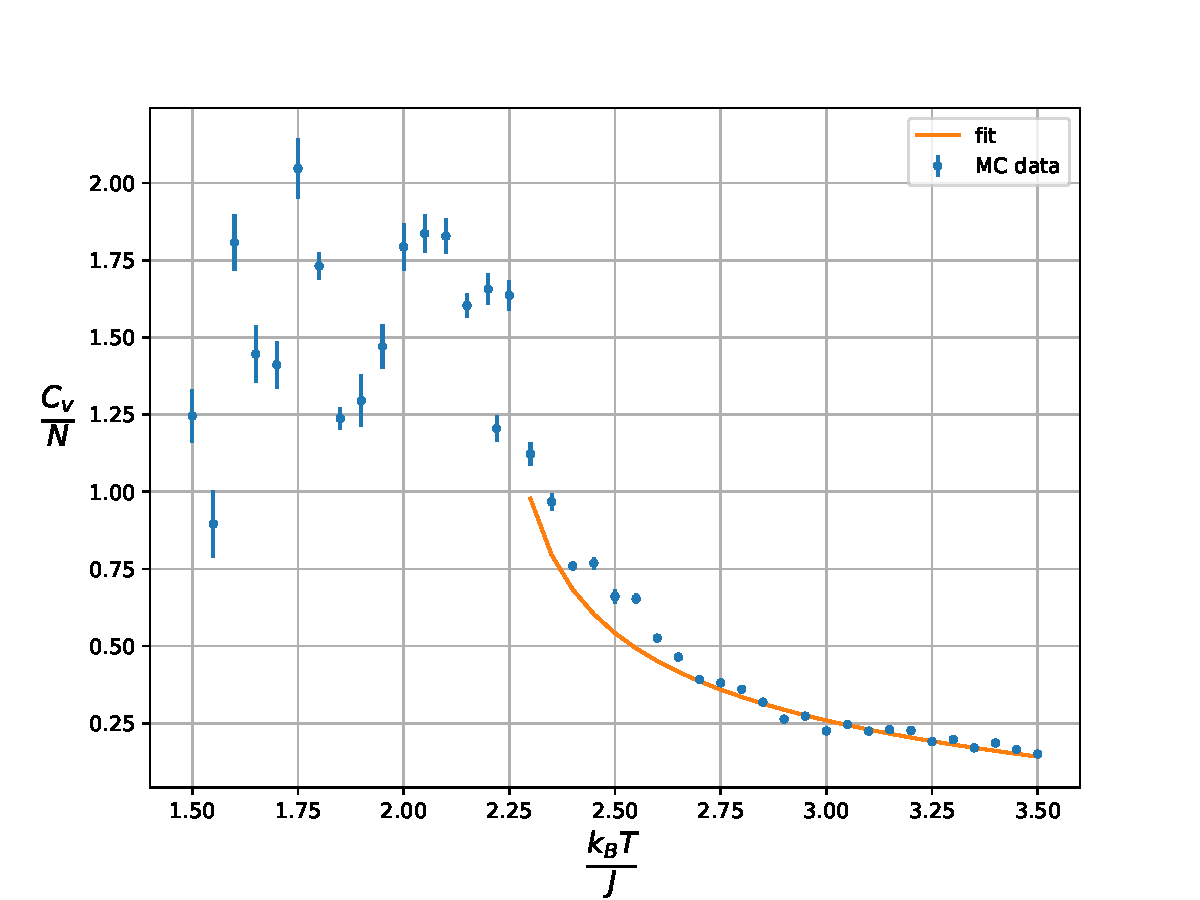
\includegraphics[scale=0.5,page=1]{multipage.pdf}
\caption{$C_v (T)$ for $h=0$}
\end{figure}

\begin{figure}[H]                                   
\centering                                       
\includegraphics[scale=0.5,page=3]{multipage.pdf}
\caption{$M^2 (T)$ for $h=0$}                    
\end{figure}                                     

The roughness of the estimate via simple fit of the functions defining the critical
exponents is due to the fact that the Monte Carlo simulations tend to struggle near critcal
point where observables' values oscillate excessively, reducing then the effectiveness
of the averaging process of the Monte Carlo method. 

\begin{figure}[H]
\centering                                       
\includegraphics[scale=0.5,page=2]{multipage.pdf}
\caption{$C_v (T)$ for $h \neq 0$}                    
\label{fig:cvh}
\end{figure}                                     

Observable values for the ordering field $h\neq 0$ are reported in the graphs below. 
The effect of the field is to keep the order in the spin configuration, raising the
value of the critical point, as can be seen in figure~\ref{fig:cvh}, and to keep
a considerable magnetization after the transistion, as can be see in 
figure~\ref{fig:m2h}.

\begin{figure}[H]
\centering                                       
\includegraphics[scale=0.5,page=4]{multipage.pdf}
\caption{$M^2 (T)$ for $h \neq 0$}                    
\label{fig:m2h}                               
\end{figure}                                     

A study of the magnetization at the critical temperature for different values of the
ordering field is carried to estimate the critical exponent $\delta$. The results are 
reported in figure~\ref{fig:m2hh}.

\begin{figure}[H] 
\centering 
\includegraphics[scale=0.5,page=5]{multipage.pdf}
\caption{$M^2 (h)$ for $T=T_c$}                    
\label{fig:m2hh}
\end{figure}                                     

A table with the results of the fits and the corrisponding critical exponents is
reported below. Theoretical and experimental values for the model are also 
reported. \footnote{for tables of theoretical and experimental values see \cite
{pathria1972statistical}}

\begin{table}[h]
\resizebox{\textwidth}{!}{
\begin{tabular}{|c|c|c|c|c|c|}
\hline
& $\alpha$ & $\beta$ & $\delta$ & $\gamma$ & $\nu$ \\ \hline
Theorical values &  & $0.362 \pm 0.012$ & $4.82 \pm 0.12$ & $1.39 \pm 0.01$ & $0.705 \pm 0.005$ \\ \hline
Experimental values & 0.0-0.2 & 0.3-0.36 & 4.2-4.8 & 4.2-4.8 & 0.62-0.68 \\ \hline
Monte Carlo simulation & $0.201 \pm 0.004$ & $0.438 \pm 0.001$ & $3.86 \pm 0.09$ & $0.654 \pm 0.008$ & $1.08 \pm 0.03$ \\ \hline
$\chi^2_r$ & $\simeq 7\cdot 10^5$ & $\simeq 1\cdot 10^{12}$ & $\simeq 3 \cdot 10^{12}$   &  &    \\ \hline
\end{tabular}}
\end{table}

The values of $\alpha$, $\beta$ and $\delta$ have been obtained directly, while $\gamma$
and $\nu$ have been obtained by $\alpha$, $\beta$ and $\delta$ with the hyperscale
realtions in equation~\ref{eq:hyper}.

By looking at the values of the reduced chi squared it seems obvious that these
fit have to be rejected. Such big values are determined both by an underestimate
of the errors on observables, mainly in the temperature region near the critical 
point, and by a not very good choice of the fitting functions. Anyway a kind of 
agreement, due mainly to the not so precise experimental values, appears beetwen 
experimantal values and the one coming from this work. So it can be said that
the macroscopic behaviour and properties of systems which can be described by the
3 dimensional XY model have been shown.
